\section{SSLStrip}

%%%%%%%%%%%%%%%%%%%%%%%%%%%
%  Principes              %
%%%%%%%%%%%%%%%%%%%%%%%%%%%

\begin{frame}[fragile]{Attaque SSLStrip - principes}
  \begin{block}{But de l'attaque}
    \begin{itemize}
    \item Récupérer le trafic en clair
    \end{itemize}
  \end{block}
  \begin{block}{Fonctionnement}
    \begin{enumerate}
      \item Modifier la réponse HTTP du serveur
      \item Remplacer les liens HTTPS en HTTP
      \item Sauvegarde en mémoire
      \item Requête POST = Expiration cookies
    \end{enumerate}
  \end{block}
\end{frame}

%%%%%%%%%%%%%%%%%%%%%%%%%%%
%  Attaque générale       %
%%%%%%%%%%%%%%%%%%%%%%%%%%%

\begin{frame}{Attaque SSLStrip}
    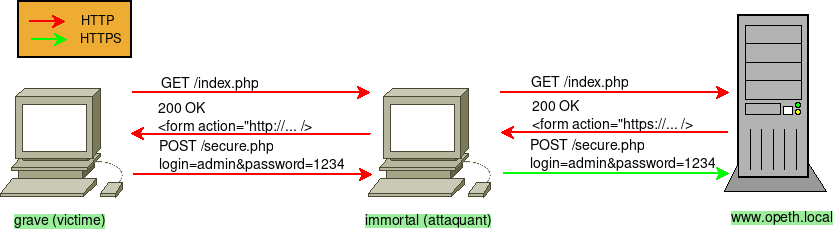
\includegraphics[width=\linewidth]{../medias/sslstrip/attack.png}
\end{frame}

%%%%%%%%%%%%%%%%%%%%%%%%%%%
%  SSLStrip démo          %
%%%%%%%%%%%%%%%%%%%%%%%%%%%

\begin{frame}{Attaque SSLStrip - démonstration}
  % deux images du code source HTML (cf rapport)
  % essayer de mettre des flèches
\end{frame}
